{
\renewcommand{\baselinestretch}{1.0}
\begin{figure}[t]
\begin{center}
\subfigure[Scaling a PDS sort benchmark up to 25 nodes.]{
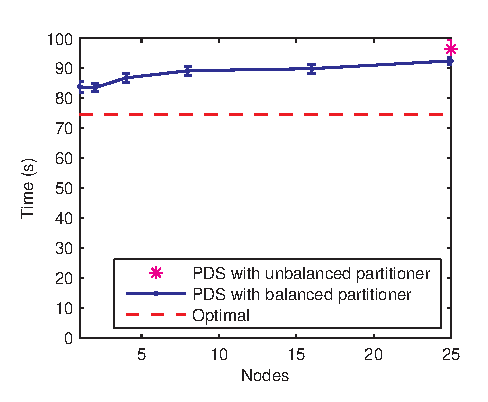
\includegraphics{fig_pds_sort1.eps}
\label{fig:pds:sort1:scale}
}
\subfigure[Time breakdown.]{
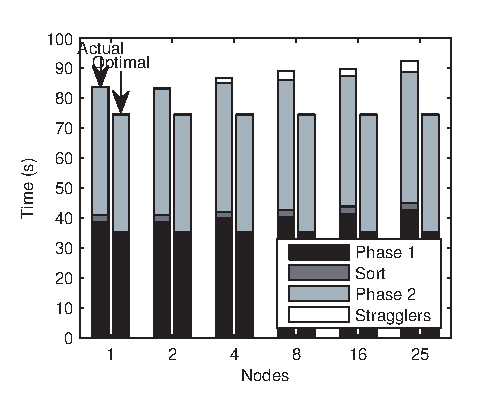
\includegraphics{fig_pds_breakdown1.eps}
\label{fig:pds:sort1:breakdown}
} \minicaption{Using Parallel DataSeries to sort up to 100~GB, it is
  possible to approach within 12-24\% of the optimal sort times as
  predicted by our performance model} {PDS scales well for an
  in-memory sort with 4~GB per node up to 25 nodes in {\bf (a)},
  although there is a small time increase starting around 4 nodes due
  to network effects.  Also shown for the 25 node case is the
  performance of our older, unbalanced partitioner, which had an
  additional 6\% performance overhead from optimal.  A breakdown of
  time in {\bf (b)} shows that the time increases at scale are mostly
  in the first phase of a map-reduce dataflow, which includes the
  network data shuffle, and in the time nodes spend waiting for
  stragglers due to effects of skew. }

\label{fig:pds:sort1}
\end{center}
\end{figure}
}

